%%%%%%%%%%%%%%%%%%%%%%%%%%%%%%%%%%%%%%%%%%%%%%%%%%%%%%%%%
%%%
%%%  第5章
%%%  結論
%%%
%%%%%%%%%%%%%%%%%%%%%%%%%%%%%%%%%%%%%%%%%%%%%%%%%%%%%%%%%
\section{Conclusion}

In this research, we have focused on the development of self-recognition and modular control capabilities for Moonbot, a modular legged robot. By providing adaptability to different configurations, Moonbot uses internal sensor to demonstrate the ability to recognize itself and its potential to operate in various configurations. The ROS2-based control framework implemented enables seamless integration of different modules and additional sensors, paving the way for future advancements in Moonbot's capabilities.

Furthermore, the development of a high-level controller for Moonbot's quadruped configuration, both in simulation and real-world scenarios, showcases its operational versatility and robustness. These achievements mark significant milestones towards autonomous and adaptable robotic systems for lunar exploration and beyond.

\section{Future Improvements Plan}

Looking ahead, future work will focus on enhancing Moonbot's control strategies and adaptability through the implementation of reinforcement learning (RL) algorithms, particularly tailored for the lunar surface environment. RL has shown promise in enabling robots to learn and adapt to complex and dynamic environments by continuously improving their decision-making processes based on feedback from the environment. In the context of legged robots, RL algorithms can be utilized to optimize locomotion patterns and adapt to varying terrain conditions, ultimately enhancing the robot's mobility and efficiency. Many researchers have driven into this new strategies to control legged robot, for example, Anymal from ETH Zurich \cite{anymalRL}, \cite{anymalDRL}.

\begin{figure}[t]
  \centering
  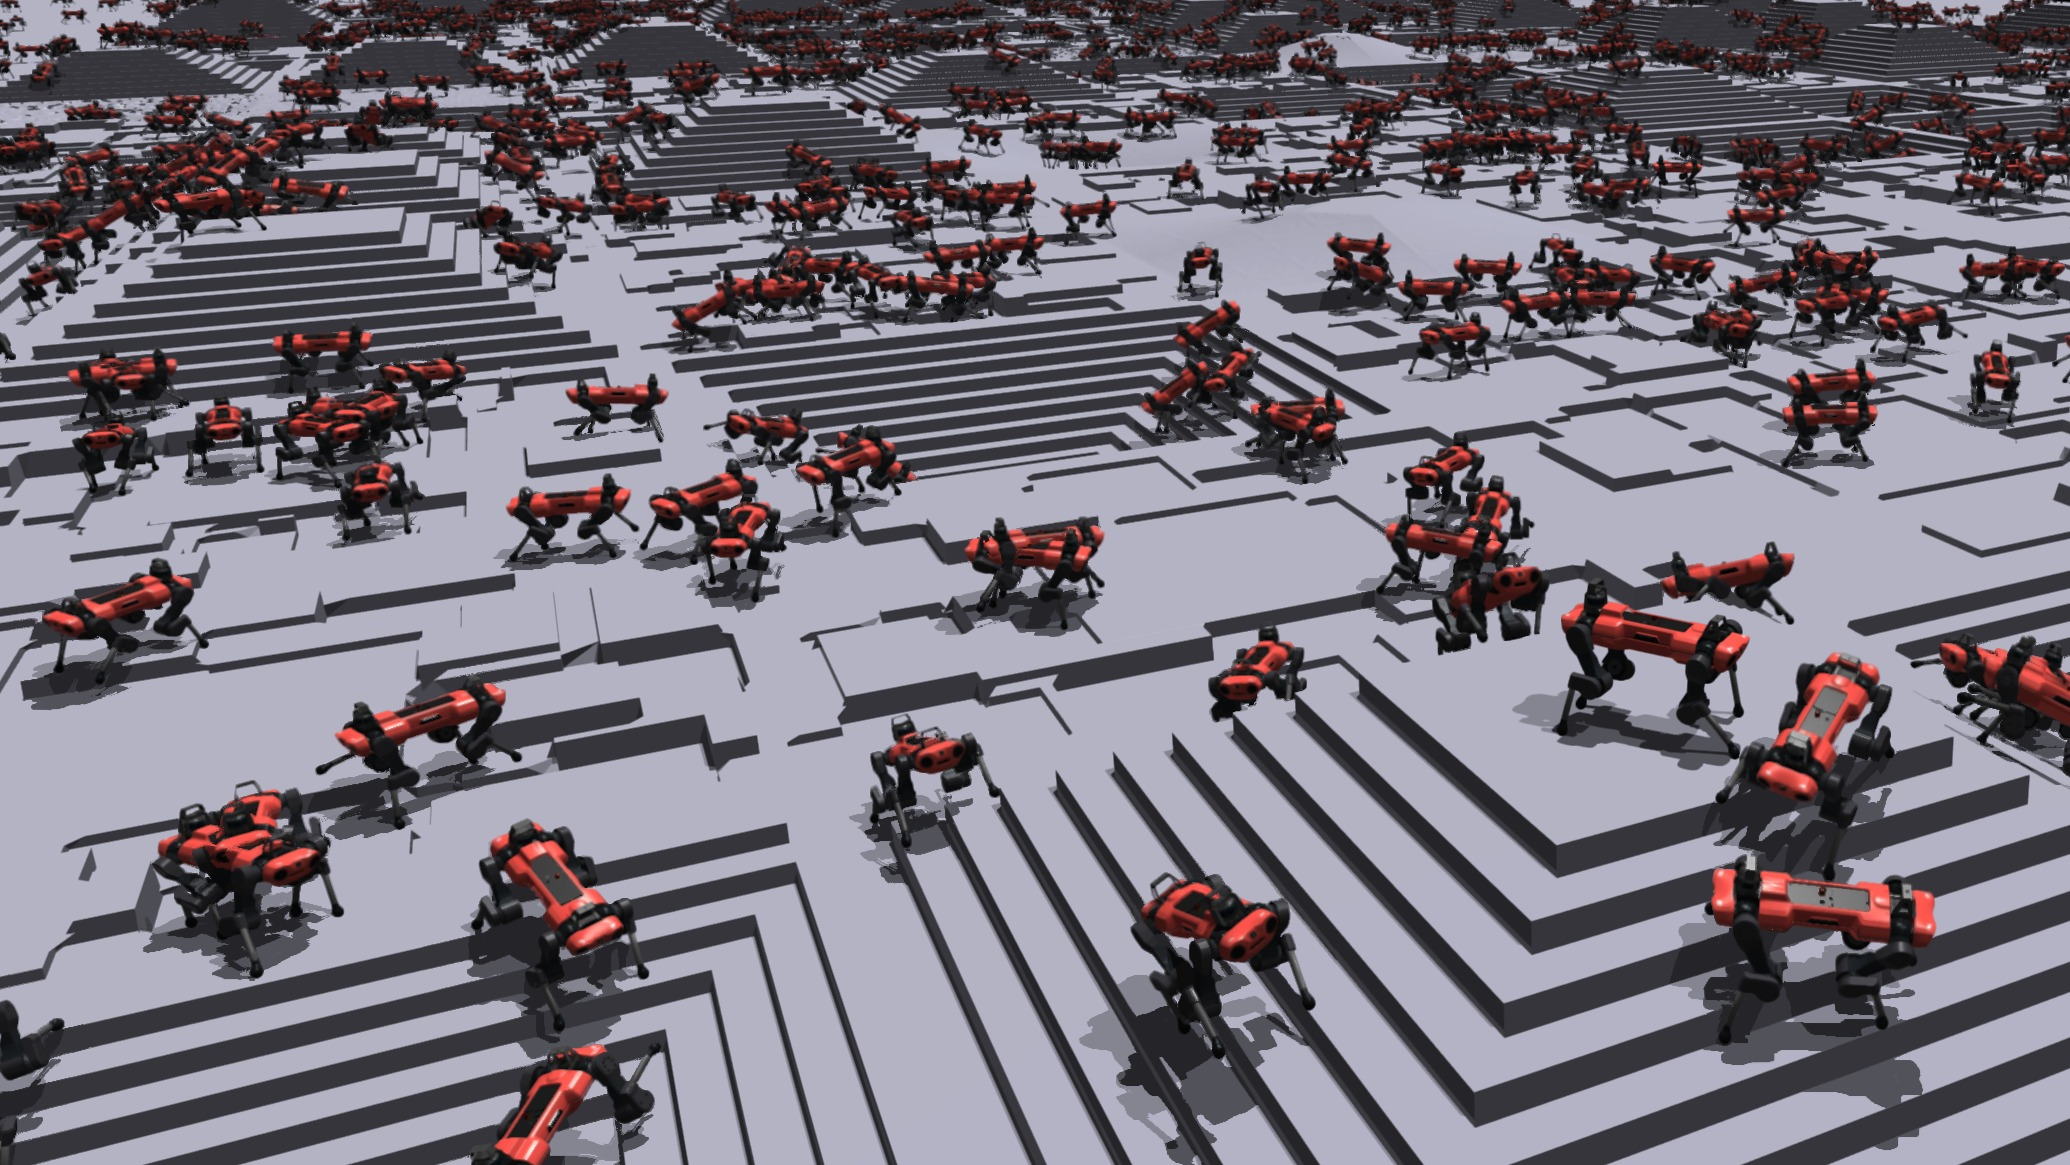
\includegraphics[width=140mm]{./fig/chap5/isaacgym.jpg}
  \vspace{2mm}
  \caption{Anymal robot walking training in Isaac Gym environment. \cite{legged_gym_git}}\label{anymalgym}
\end{figure}

Furthermore, in the modularity side, the application of deep reinforcement learning (DRL) algorithms will be investigated to optimize the design process of modular legged robots \cite{modularDRL}, \cite{modularlegDRL}. DRL techniques, which leverage deep neural networks to approximate complex functions, offer the potential to revolutionize the way legged robots are designed and controlled. By using DRL, Moonbot and similar robots can autonomously learn and refine their locomotion strategies, leading to more agile and robust robotic systems.\\

% \begin{figure}[ht]
%   \centering
%   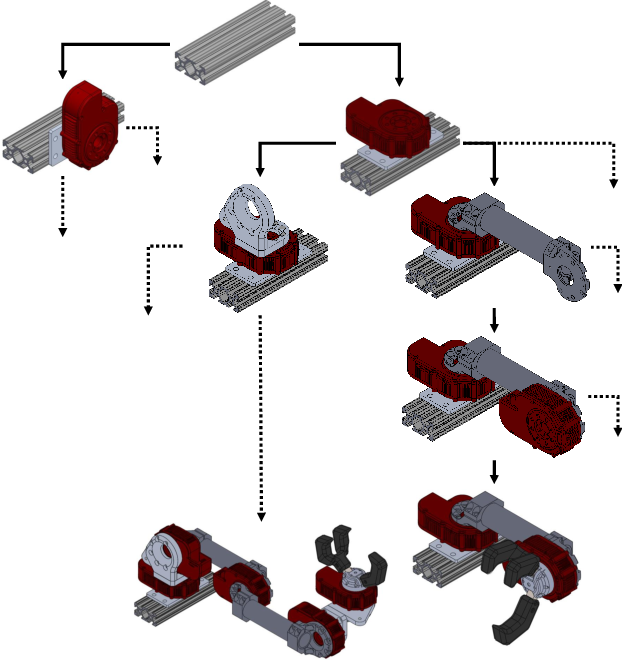
\includegraphics[width=90mm]{./fig/chap5/modularDRL.png}
%   \vspace{2mm}
%   \caption{Modular manipulator design tree, synthesized by deep reinforcement learning. \cite{modularDRL}}\label{modularDRL}
% \end{figure}



The integration of reinforcement learning techniques into the control and design processes of modular legged robots represents a significant step towards achieving autonomous operation in challenging environments, such as lunar surfaces. By leveraging RL and DRL algorithms, Moonbot and future generations of legged robots can overcome obstacles, navigate complex terrains, and accomplish tasks with greater efficiency and adaptability.

In conclusion, the combination of reinforcement learning, modular robotics, and space exploration holds immense potential for advancing the field of robotics and unlocking new capabilities for autonomous systems. By bridging the gap between theoretical research and practical application, we can pave the way for the next generation of robotic explorers, capable of operating effectively in the harsh and unpredictable environments of space.

\begin{figure}[t]
    \centering
    \begin{subfigure}{1.0\textwidth}
        \centering
        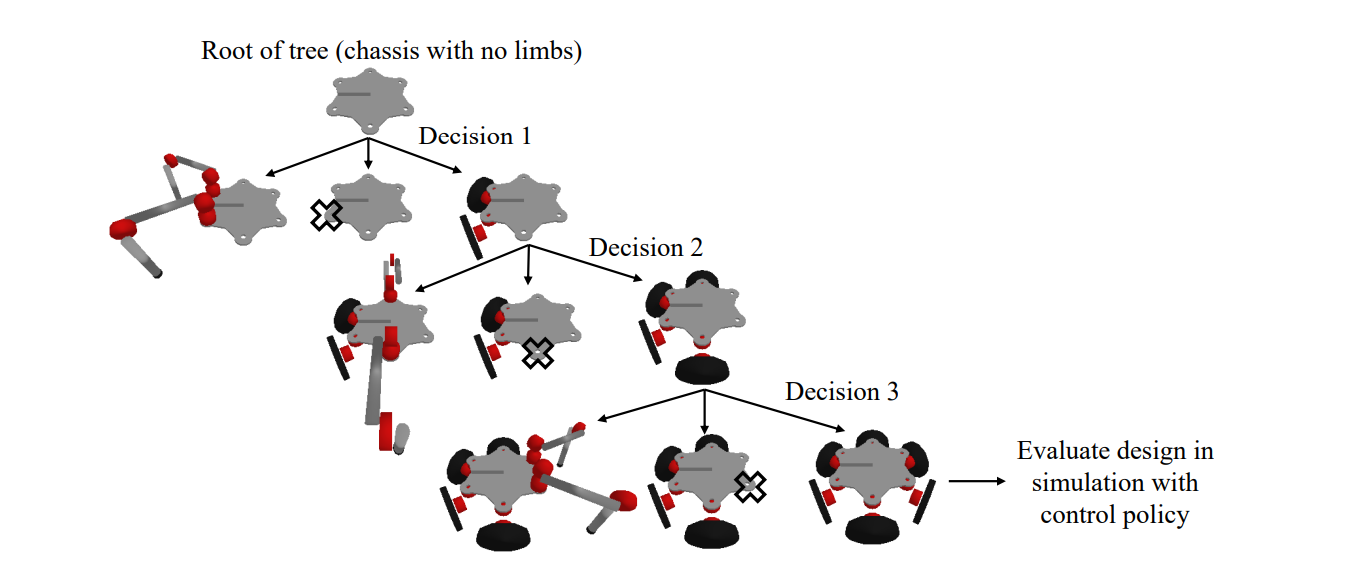
\includegraphics[width=140mm]{./fig/chap5/modularlegDRLtree.png}
        \caption{Design space tree for modular mobile robot, using deep neural network.}
        \label{moduleDRLtree}
    \end{subfigure}
    % \hfill
    \\
    \begin{subfigure}{1.0\textwidth}
        \centering
        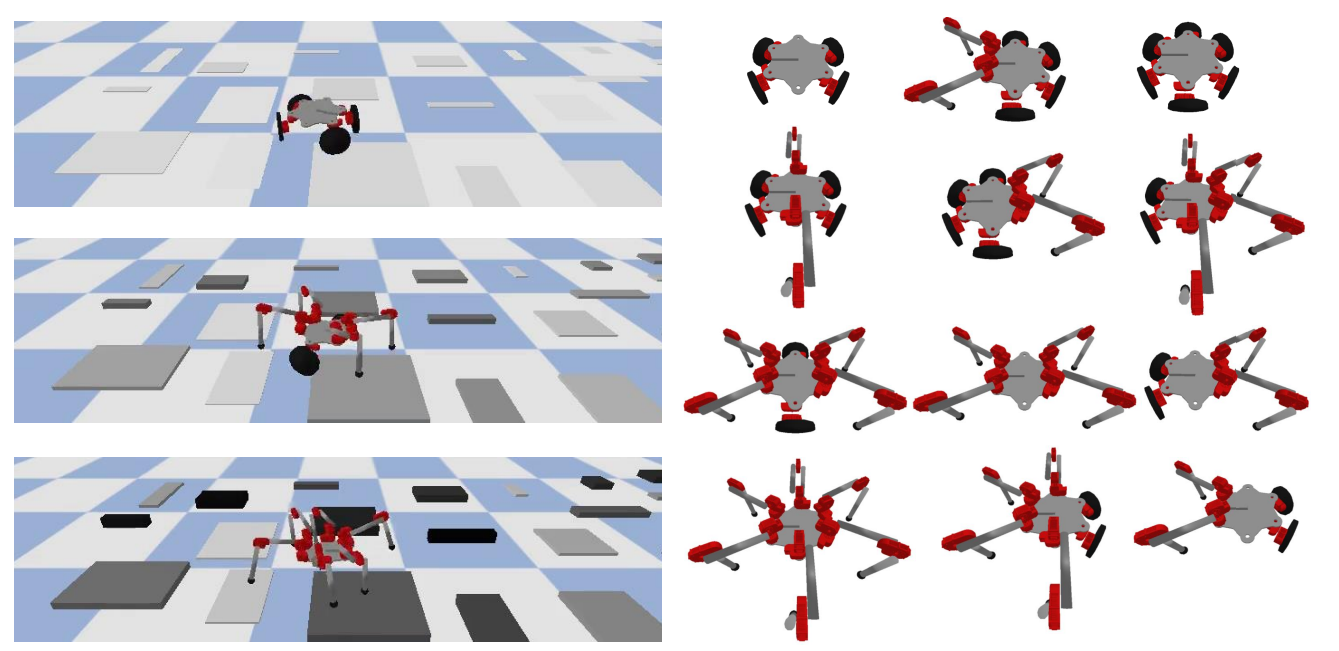
\includegraphics[width=140mm]{./fig/chap5/modularlegDRL.png}
        \caption{Evaluation of modular designs in simulation across terrains of varying roughness, showcasing the adaptability of different robot configurations.}
        \label{modularDRL}
    \end{subfigure}
    \vspace{2mm}
    \caption{Modular mobile robot design selection with deep reinforcement learning. \cite{modularlegDRL}}
    \label{DRLmodular}
\end{figure}


%%% EOF %%%